% ============================ 00 总览 ============================

\begin{frame}{汇报内容与组织}
  \begin{columns}[t]
    \begin{column}{0.48\textwidth}
      \begin{block}{视角一：前向推理（部署时）}
        \small
        \begin{itemize}\tight
          \item 候选从哪里来：\textbf{固定锚点}
          \item 网络预测什么：\textbf{有界修正量}
          \item 曲线从哪里来：\textbf{解析 BVP}
          \item 选哪一条：预测评分 $\arg\min$
          \item 时序：重规划 / 参考输出 / 执行
        \end{itemize}
      \end{block}
    \end{column}
    \begin{column}{0.48\textwidth}
      \begin{block}{视角二：引导训练（离线时）}
        \small
        \begin{itemize}\tight
          \item 监督信号来自哪里：\textbf{特权地图}
          \item 代价函数的三项分解
          \item 外部数值梯度如何进入网络
          \item 评分支路：回归什么、为何暂停梯度
          \item 候选筛选、特权学习与数据
        \end{itemize}
      \end{block}
    \end{column}
  \end{columns}

  \vspace{0.3em}
  \begin{reading}[阅读约定（沿用笔记的标注规则）]
    \small
    蓝色块为原文可查证的结论；绿色块为便于理解而构造的教学数字；
    橙色块为本报告的整理与推论，\textbf{不代表原文陈述}。
  \end{reading}
\end{frame}

\begin{frame}{论文基本信息}
  \small
  \begin{columns}[t]
    \begin{column}{0.52\textwidth}
      \begin{block}{文献}
        \begin{itemize}\tight
          \item 标题：\emph{You Only Plan Once: A Learning-Based One-Stage Planner With Guidance Learning}
          \item 作者：Junjie Lu, Xuewei Zhang, Hongming Shen, Liwen Xu, Bailing Tian（天津大学）
          \item 出处：IEEE RA-L, 2024, 9(7): 6083--6090
          \item DOI：\texttt{10.1109/LRA.2024.3399589}
          \item 代码：\texttt{github.com/TJU-Aerial-Robotics/YOPO}
        \end{itemize}
      \end{block}
    \end{column}
    \begin{column}{0.44\textwidth}
      \begin{block}{方法概述}
        \footnotesize
        把传统规划的三段式流水线——\textbf{感知建图、前端搜索、后端优化}——
        压进\textbf{一次网络前向}：
        用运动基元铺开搜索空间，用网络预测基元的修正量与评分，
        用\textbf{外部代价的数值梯度}当作训练监督。
      \end{block}
    \end{column}
  \end{columns}

  \vspace{0.2em}
  \begin{paperfinding}[本报告聚焦的两问]
    \footnotesize
    ① 候选轨迹的生成方式；② 单一规划代价同时训练轨迹输出与评分输出的机制。
  \end{paperfinding}
\end{frame}

\begin{frame}{研究背景：传统三段式规划流程的局限}
  \begin{columns}[c]
    \begin{column}{0.46\textwidth}
      \small
      \textbf{传统链路：}
      \begin{center}
      \begin{tikzpicture}[node distance=3mm, every node/.style={font=\scriptsize, align=center}]
        \node[draw=yopoblue, fill=yopopale, rounded corners, inner sep=3pt] (a) {感知\\建图};
        \node[draw=yopoblue, fill=yopopale, rounded corners, inner sep=3pt, right=of a] (b) {前端\\搜索};
        \node[draw=yopoblue, fill=yopopale, rounded corners, inner sep=3pt, right=of b] (c) {后端\\优化};
        \node[draw=yopoorange, fill=yopowarm, rounded corners, inner sep=3pt, right=of c] (d) {控制};
        \draw[-{Latex}] (a)--(b); \draw[-{Latex}] (b)--(c); \draw[-{Latex}] (c)--(d);
      \end{tikzpicture}
      \end{center}
      三段各自可解释，但\textbf{延迟叠加}；高速飞行时致命。

      \vspace{0.4em}
      \textbf{另一个难点是多模态性：}面对同一障碍时，向左与向右绕行可能
      \textbf{同样可行}。
      将多个解压缩进单一回归输出，会得到两种策略之间的\textbf{折中解}。
    \end{column}
    \begin{column}{0.5\textwidth}
      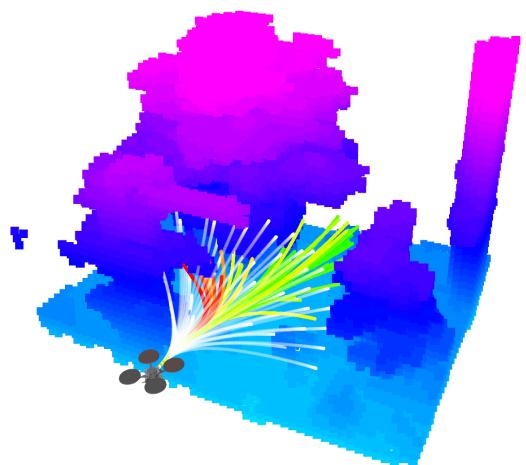
\includegraphics[width=\linewidth]{figures/01_anchor_exploration.jpg}
      \begin{center}
      \scriptsize\color{yopogray}
      原文 Fig.~1：运动基元（白线）作为锚点铺满解空间；\\
      按评分着色的预测曲线为优化结果
      \end{center}
    \end{column}
  \end{columns}
\end{frame}

\begin{frame}{方法概述：单次前向传播的规划流程}
  \begin{columns}[c]
    \begin{column}{0.6\textwidth}
      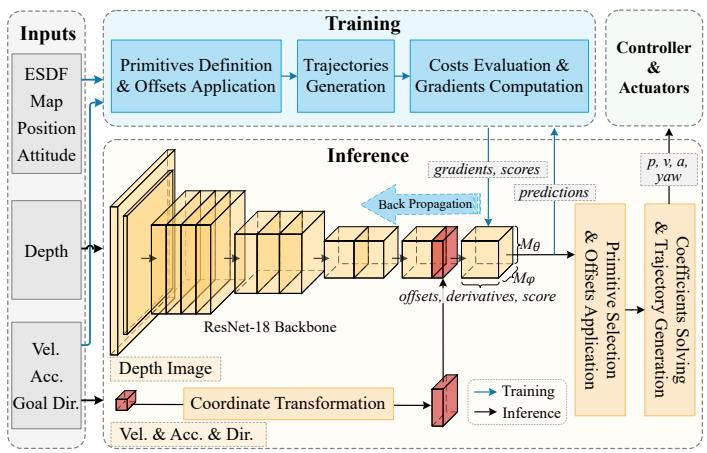
\includegraphics[width=\linewidth]{figures/03_system_overview.jpg}
      \begin{center}\scriptsize\color{yopogray}
      原文 Fig.~3：深度图 + 当前状态 + 目标方向 $\to$ 每个基元的
      偏移、终端导数、评分；\textbf{训练时}由 ESDF 计算代价与梯度
      \end{center}
    \end{column}
    \begin{column}{0.38\textwidth}
      \small
      \begin{itemize}\tight
        \item 感知 $\to$ ResNet-18 主干
        \item 前端 $\to$ 15 个基元锚点（\textbf{预定义、不占算力}）
        \item 后端 $\to$ 网络预测的终端状态
              $+$ 五次多项式解析求解
      \end{itemize}
      \begin{reading}
        \scriptsize
        图上“Training / Inference”两条支路共用同一个网络：
        差别在于训练阶段增加了查询地图并计算梯度的评价环节。
      \end{reading}
    \end{column}
  \end{columns}
\end{frame}

\begin{frame}{坐标系定义与符号约定}
  \small
  \begin{columns}[t]
    \begin{column}{0.5\textwidth}
      \begin{block}{两个坐标系}
        \begin{itemize}\tight
          \item \textbf{机体系（body frame）}：网络输入/输出与轨迹表示所在系。
                用机体系可避免网络输出位置与姿态（降维）。
          \item \textbf{基元系（primitive frame）}：第 $(i,j)$ 个锚点自己的坐标系。
                \textbf{只用于把状态与终端导数“本地化”}，不改变物理量。
        \end{itemize}
      \end{block}
    \end{column}
    \begin{column}{0.46\textwidth}
      \begin{block}{符号速查}
        \scriptsize
        \begin{tabular}{@{}ll@{}}
          \toprule
          $D$ & 深度图 \\
          $\hat{\mathbf g}$ & 网络输入的目标单位方向 \\
          $\mathbf g_{\mathrm{local}}$ & 代价里的临时目标点 \\
          $(r,\theta_j,\varphi_i)$ & 基元球坐标参数 \\
          $\mathbf y^{\mathrm{traj}}$ & 9 维原始轨迹输出 \\
          $\mathbf q$ & 解码后的终端状态 $\mathbf p_T,\mathbf v_T,\mathbf a_T$ \\
          $\hat s$ / $J$ & 预测评分 / 外部计算的代价 \\
          $\mathbf c_\mu$, $M(T)$ & 单轴多项式系数、边界映射矩阵 \\
          \bottomrule
        \end{tabular}
      \end{block}
    \end{column}
  \end{columns}

  \begin{reading}[维度约定的统一]
    \small
    本报告图像尺寸记为“宽 $\times$ 高”，张量采用 NCHW 布局。
    原文的 $M_\varphi\times M_\theta\times 10=5\times3\times10$
    按“水平、竖直、通道”排列，对应同样的 15 个候选。
  \end{reading}
\end{frame}
